\section{Compatible seeds, geometric doubling, and sparse families}
\label{fam:section}

The second extension mechanism inserts a whole collection of lines near
a distinguished support.  It belongs to Bartholdi, Blanc, and Loisel
(BBL)~\cite{bbl2008}; it is fundamentally different from the one-line
exterior operation of Section~\ref{ext:section}.  The present work supplies
explicit compatible seeds, an actual one-step geometric Lean proof, and
finite certificates at considerably larger orders.  The distinction
between a published-theorem consequence and a completed recursive Lean
theorem is maintained throughout.

\subsection{The exact one-step theorem}

Let $q=4r$ with $r\geq5$, put $\alpha=\pi/q$, and take
\begin{equation}
  0<\varepsilon<\tan(\alpha/2).
  \label{fam:epsilon}
\end{equation}
Define $q$ ordered intercepts, indexed from zero, by
\begin{equation}
 a_j=
 \begin{cases}
 \tan((j-q/2+1)\alpha),&0\leq j<q/2-1,\\
 -\varepsilon,&j=q/2-1,\\
 \varepsilon,&j=q/2,\\
 \tan((j-q/2)\alpha),&q/2<j<q.
 \end{cases}
 \label{fam:old-grid}
\end{equation}
In particular, the extreme intercepts are $-\cot\alpha$ and
$\cot\alpha$.  The two central intercepts replace the repeated zero that
would otherwise occur in this grid.

\begin{definition}[Compatible tangent-grid seed]
\label{fam:compatible}
A seed at $(q,\varepsilon)$ consists of $Y_0:y=0$ and the $q$ lines
$L_j:y=m_j(x-a_j)$, with the following properties: the arrangement is
simple; every interval $[a_j,a_{j+1}]$ on $Y_0$ supports the triangular
cell with supports $Y_0,L_j,L_{j+1}$; and the central apex
$L_{q/2-1}\cap L_{q/2}$ lies above $Y_0$.  A counted seed additionally
carries a list of distinct actual triangular cells whose length is at
least $T$.
\end{definition}

Simplicity already requires all $m_j$ to be nonzero and pairwise distinct.
The distinguished-line condition is a substantial geometric restriction,
not a consequence of having a large total count.  It is precisely why
an arbitrary optimal arrangement cannot simply be used as a repeatable
BBL seed.

\begin{theorem}[Fully verified geometric doubling]
\label{fam:doubling}
Suppose $q=4r\geq20$ and \eqref{fam:epsilon} holds.  A compatible
tangent-grid seed with at least $T$ certified triangles gives a simple
real straight-line arrangement of $2q+1$ lines with at least
\begin{equation}
  T+q^2
  \label{fam:gain}
\end{equation}
triangles.
\end{theorem}

The precise formal theorem is \texttt{BBLDoubling.doubling}.  It assumes
the actual old line equations, simplicity, each distinguished triangle,
the positive central height, and a duplicate-free triangle list.  It
does not assume a future crossing order, a list of future empty
triangles, or a triangle-count recurrence.  Its conclusion is an actual
\texttt{SimpleLowerBound}; the generic proof uses only the standard Lean
logical axioms.  The numerical doubling principle is BBL's.  The
contribution here is its completed geometric proof for these explicit
hypotheses, using the following two-parameter realization.

\begin{proof}[Geometric proof and its formal decomposition]
For $0\leq i<q$ set
\[
 \beta_i=-\frac\pi2+(i+\tfrac12)\alpha,
 \qquad b_i=\tan\beta_i.
\]
Adjoin the lines
\begin{equation}
 M_i:\quad y=\kappa g_i(\delta)(x-b_i),\qquad
 g_i(\delta)=\frac{2b_i}{1+b_i^2}+\frac\delta{b_i}
            =\sin(2\beta_i)+\delta\cot\beta_i.
 \label{fam:pencil}
\end{equation}
Choose $\delta>0$ sufficiently small and then $\kappa>0$ sufficiently
small relative to the fixed $\delta$ and the seed.  This order of choices
is part of the proof.  BBL's published construction uses explicit scales;
the qualitative two-scale statement here is established independently
by the formal crossing analysis, rather than inferred from those fixed
scales.

For two new lines put $t=b_i$ and $u=b_k$.  Their intersection has
$x$-coordinate independent of $\kappa$:
\begin{equation}
 X_{ik}(\delta)=
 \frac{2tu(t+u)}{2tu(1-tu)-\delta(1+t^2)(1+u^2)}.
 \label{fam:crossing}
\end{equation}
When $tu\ne1$, its limit is the reduced tangent
$(t+u)/(1-tu)=\tan(\beta_i+\beta_k)$, and the exact displacement is
\begin{equation}
 X_{ik}(\delta)-\frac{t+u}{1-tu}
 =\frac{\delta(t+u)(1+t^2)(1+u^2)}
 {[2tu(1-tu)-\delta(1+t^2)(1+u^2)](1-tu)}.
 \label{fam:displacement}
\end{equation}
For sufficiently small positive $\delta$ its nonzero sign is that of
$(t+u)tu$.  If $tu=1$, the crossing diverges along the specified exterior
ray as $\delta\downarrow0$; if $t+u=0$, its coordinate is exactly zero.
Thus neither exceptional case is hidden inside a continuity argument
with a vanishing denominator.

The reduced tangents, the old intercepts, the new half-grid intercepts,
and $-\varepsilon,0,\varepsilon$ determine a strictly ordered finite
system of cuts.  Equations~\eqref{fam:crossing}--\eqref{fam:displacement}
place every new--new crossing in its prescribed cut interval.  Taking
$\delta$ in the intersection of the finitely many resulting positive
neighborhoods also makes the new slope factors nonzero and distinct.
For fixed such $\delta$, each old--new intersection tends to the
corresponding old intercept as $\kappa\to0$.  Finite continuity then
realizes all the prescribed strict crossing comparisons simultaneously.
Small $\kappa$ separates old and new slopes.  Injectivity along each new
crossing row excludes new triple intersections; old simplicity excludes
the remaining ones.  This proves actual simplicity and crossing order.

The count can now be separated from trigonometry.  Treat the $q$ new lines
and $Y_0$ as $q+1$ auxiliary supports.  The integer row model places old
support $j$ at key $4j+2$.  A pair of auxiliary supports with crossing key
$z$ yields a mixed triangle with old support $j$ when
\begin{equation}
  |z-(4j+2)|<4.
  \label{fam:neighbors}
\end{equation}
Every auxiliary pair has two such old neighbors, except for at most $q$
exterior pairs, each of which has one.  Hence the number is at least
\begin{equation}
 2\binom{q+1}{2}-q=q^2.
 \label{fam:mixed-count}
\end{equation}
The row inequalities make two sides consecutive on their supports.
The two-side emptiness lemma proves that the corresponding triangle is
an actual empty cell.  The supporting triples are distinct.  Thus
\eqref{fam:mixed-count} counts genuine triangles, not merely local
crossing patterns.

It remains to preserve the seed's contribution.  An old triangle not
using $Y_0$ has a strict half-plane sign against $Y_0$; all new lines
converge to $Y_0$, so its three vertex signs persist for sufficiently
small $\kappa$.  The old triangles with a side on $Y_0$ require a different
argument.  Saturation forces consecutive old apices to have opposite
heights.  The positive central apex fixes the alternating parity.
The crossing order identifies a new cap support for each noncentral
distinguished triangle.  On both cap endpoints, every new line has the
parity-correct weak sign; strict signs against other old supports
persist by continuity.  This replaces each such old triangle by one
empty triangle with the same two old supports.  The central triangle
itself is retained.  The finite cap and noncap requirements can again
be satisfied by one common positive $\kappa$.

Finally, these $T$ retained or replaced triangles have at least two old
nonhorizontal supports, while the $q^2$ mixed triangles have two
auxiliary supports.  The supporting triples cannot coincide.  Their
union is a duplicate-free witness of length at least $T+q^2$.
\end{proof}

The recurrence preserves the certified segment deficit:
\begin{equation}
 \Delta(q,T)=q^2-1-3T,\qquad
 \Delta(2q,T+q^2)=\Delta(q,T).
 \label{fam:deficit-preserved}
\end{equation}
Here the equality concerns the transported lower count; if the output
has additional uncounted triangles, its actual defect can be smaller.
Thus doubling amplifies a compatible seed to larger orders while
preserving its certified constant deficit.  A smaller-defect seed or a
new source of additional triangles is needed to improve that deficit.

\subsection{The compatible eleven-line realization}

The useful eleven-line count is $32$, an existing result; the search
started from the Honma-based construction displayed by
Savchuk~\cite{savchuk2025}.  The additional work here is an explicit
realization compatible with the BBL grid for arbitrarily small positive
central separation.  Take $Y_0:y=0$ and
\begin{equation}
 x-v_jy=a_j,\qquad
 (v_0,\ldots,v_9)=\tfrac1{10}(15,-2,14,1,4,-4,5,-3,12,-5),
 \label{fam:seed11-slopes}
\end{equation}
where
\begin{equation}
 (a_0,\ldots,a_9)=
 (-\tan\tfrac{4\pi}{10},-\tan\tfrac{3\pi}{10},
 -\tan\tfrac{2\pi}{10},-\tan\tfrac{\pi}{10},
 -\varepsilon,\varepsilon,
 \tan\tfrac{\pi}{10},\tan\tfrac{2\pi}{10},
 \tan\tfrac{3\pi}{10},\tan\tfrac{4\pi}{10}).
 \label{fam:seed11-grid}
\end{equation}
For every $0<\varepsilon\leq10^{-5}$ the seed is simple, has at least
32 certified triangles, and has all nine distinguished triangles.
Its central slopes are $5/2$ and $-5/2$ and its central height is
$5\varepsilon/2>0$.

The stability check is finite but uniform in $\varepsilon$.  The
determinant for a triple of nonhorizontal lines is affine in the
intercepts and therefore affine in $\varepsilon$:
\[
 D_{ijk}=(a_j-a_k)v_i+(a_k-a_i)v_j+(a_i-a_j)v_k.
\]
Exact rational enclosures for the four tangent values and endpoint
sign checks certify the whole interval.  The first certificate used
outward rational interval arithmetic; the subsequent Lean theorem uses
proved trigonometric enclosures and the parametric certificate soundness
theorem.  The limit $\varepsilon=0$ is used only to bound expressions;
it is not presented as a simple arrangement.  Five visible pairs for
$w=(10,-13)$ are also proved uniformly, giving the actual exterior bound
$12:37$ by Theorem~\ref{ext:realization}.

\begin{figure}[tb]
\centering
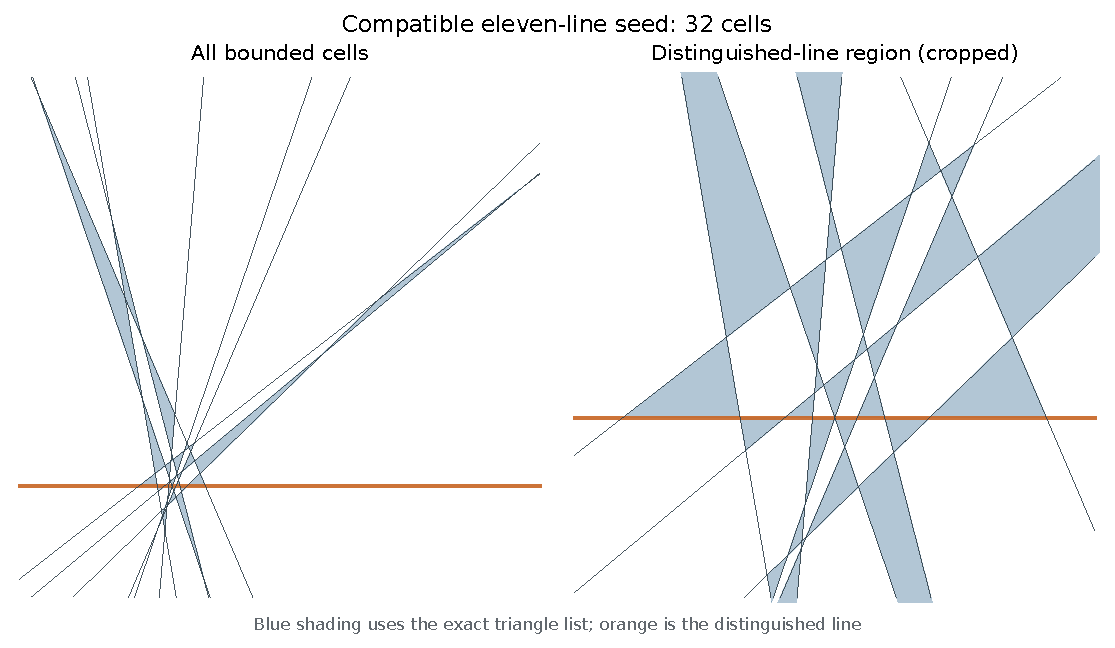
\includegraphics[width=0.88\linewidth]{figures/seed-11.pdf}
\caption{A finite rational realization of the compatible eleven-line
seed, with global and distinguished-line views.  The figure illustrates
the arrangement; the all-small-parameter
claim is certified by exact determinant and half-plane inequalities,
not by the rendering.  The count $32$ is inherited from earlier work;
the compatible realization and parameter certificate are the contribution
recorded here.}
\label{fig:seed11}
\end{figure}

Using the published BBL construction, with its finite-depth choice of
the exceptional parameter, gives the ordinary mathematical family
\begin{equation}
 q_t=10\cdot2^t,\qquad N_t=q_t+1,\qquad
 \Ks(N_t)\geq T_t=\frac{100\cdot4^t-4}{3}.
 \label{fam:eleven-family}
\end{equation}
The arithmetic is
\[
 T_0=32,\quad T_{t+1}=T_t+q_t^2,
 \quad
 T_t=32+100\sum_{j<t}4^j=\frac{q_t^2-4}{3}.
\]
The BBL geometric theorem and its iteration mechanism retain their
original attribution.  The formula is one below
$\lfloor N_t(N_t-2)/3\rfloor=(q_t^2-1)/3$; at $N_0=11$ the sharper known
upper bound is already $32$~\cite{savchuk2025}.
The checkpoints $21:132$ and $41:532$ are weaker than the known
$21:133$ and $41:533$.  Thus the formula is not a record assertion at
every member.

The quantifiers matter.  For any prescribed finite depth $t$, one can
choose the starting exceptional parameter small enough for every step
up to $t$; the recorded application uses
$0<\varepsilon\leq\min\{10^{-5},(40\cdot2^t)^{-1}\}$.
A single fixed positive $\varepsilon$ working through infinitely many
steps is neither required nor claimed.  Equation~\eqref{fam:eleven-family}
is supported by the verified seed and the published BBL theorem.  It is
not yet an end-to-end infinite-family theorem in the Lean library:
Theorem~\ref{fam:doubling} starts at $q\geq20$, and its recursive witness
interface remains to be assembled as described below.

\subsection{Even companions and the stronger boundary invariant}

The arrangement in \eqref{fam:eleven-family} has defect three.  Theorem
\ref{ext:defect-theorem} therefore gives the paper-level infinite bound
\begin{equation}
 \Ks(q+2)\geq\frac{q^2-4}{3}+\frac q2-1,
 \qquad q=10\cdot2^t.
 \label{fam:even-defect}
\end{equation}
Indeed,
$g(q+1,(q^2-4)/3)=\lceil q(q-2)/(2(q+1))\rceil=q/2-1$.
The stronger value observed in all completed finite examples is
\begin{equation}
 \frac{q^2-4}{3}+\frac q2.
 \label{fam:even-strong}
\end{equation}
For $M=q+2$, equations~\eqref{fam:even-defect} and
\eqref{fam:even-strong} equal respectively
$M(M-5/2)/3-2$ and $M(M-5/2)/3-1$.
The polynomial is the relevant Blanc upper bound for \emph{simple}
arrangements in these residue classes~\cite{blanc2011}; it is not an
upper bound asserted here for unrestricted $\K(M)$, and small orders
can have sharper bounds.

\begin{proposition}[Conditional full-gain even family]
\label{fam:even-conditional}
If the compatible odd family admits at least $q/2$ visible pairs from
an admissible normal at each stage, then
\[
 \Ks(q+2)\geq\frac{q^2-4}{3}+\frac q2
 \qquad(q=10\cdot2^t).
\]
\end{proposition}

\begin{proof}
Apply Theorem~\ref{ext:realization} at each specified odd order.
\end{proof}

The working boundary argument supplies a concrete route to the premise,
rather than treating it as an unexplained numerical assumption.  Keep
$w=(10,-13)$ and require the rightmost old intercept line $R$ to have
slope $0<m_R<10/13$, with its rightmost vertex on $Y_0$.  Old visible
pairs avoiding $Y_0$ persist under a sufficiently small pencil, and at
most one visible old pair uses $Y_0$.  For $q=4r$ the proposed new pairs
are $r$ negative complementary pairs, $r-1$ positive almost-complementary
pairs, the pair formed by $Y_0$ and the rightmost new support, and a pair
formed by $R$ and the new support at
$\beta_* =\pi/4-\alpha/2$.  Their total is $q/2+1$, giving a net gain
of at least $q/2$ visible pairs after losing at most one.

The delicate last pair is governed by the strict maximum
\[
 \cot\alpha\sin(2\beta)+\cos(2\beta)-1
 =\frac{\sin(2\beta+\alpha)}{\sin\alpha}-1.
\]
On the half-grid it is uniquely maximal at $\beta_*$, with gap at least
$2\sin\alpha$ from every other index.  Its persistence under the
$\delta$ perturbation and then the scale ratio $\kappa/m_R$ is proved
for actual intersections.  The remaining assembly must compare this
maximum with all old vertices, transfer the $x$-order to $w$-order, and
preserve the rightmost-line hypothesis under reindexing.  A detailed
ordinary working proof is archived, but the completed components are
not presented here as an already assembled infinite Lean invariant.
Proposition~\ref{fam:even-conditional} makes that status explicit.

\begin{table}[tb]
\centering
\small
\begin{tabular}{rrrrrl}
\hline
$q$ & Odd order & Odd count & Even order & Even count & Verification\\
\hline
10&11&32&12&37&Lean finite witnesses\\
20&21&132&22&142&Lean finite witnesses\\
40&41&532&42&552&Lean finite witnesses\\
80&81&2132&82&2172&Lean finite witnesses\\
160&161&8532&162&8612&Lean finite witnesses\\
320&321&34132&322&34292&Two exact counters\\
640&641&136532&642&136852&See text: 642 partial\\
\hline
\end{tabular}
\caption{Explicit hybrid checkpoints.  The even column uses the stronger
finite gain $q/2$; the infinite defect guarantee is one less.  These
counts describe this family, and need not be the strongest known count
at the displayed order.  In the last row only 641 has completed both
independent exact counters.}
\label{fam:finite-table}
\end{table}

\begin{figure}[tb]
\centering
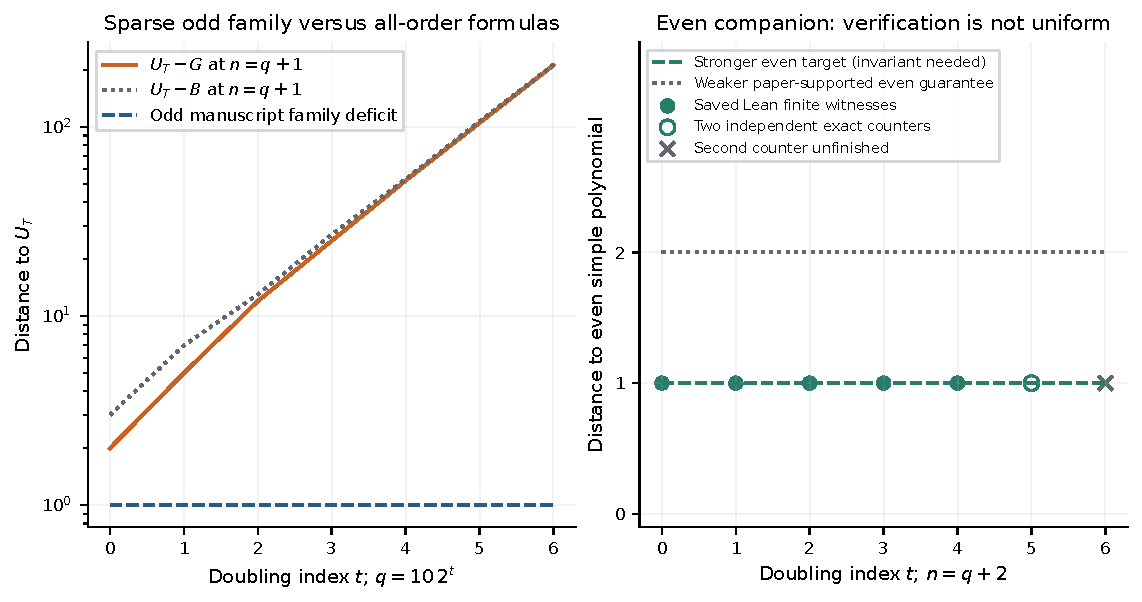
\includegraphics[width=0.88\linewidth]{figures/family-deficits.pdf}
\caption{The sparse hybrid family compared with the all-order baselines.
Odd counts are one below the classical segment bound; the stronger
even checkpoints are one below the displayed simple polynomial bound.
Finite Lean certificates, larger exact coordinate checks, and
family formulas have different verification scopes; the plot does not
turn an incomplete recursive formalization into a proved Lean theorem.}
\label{fig:family-deficits}
\end{figure}

For 321, 322, and 641 lines the adjacency counter and an independently
implemented direct half-plane-sign counter agree on $34132$, $34292$,
and $136532$ triangles, respectively, and simplicity is checked exactly.
The largest rational components have 916, 985, and 1103 decimal digits.
These are archived exact coordinate witnesses, outside the routine
finite Lean catalogue.  The 642-line coordinate file passed the adjacency
and simplicity checks, but its independent direct count was interrupted.
Its displayed value $136852$ is therefore partial computational evidence,
not a completed two-counter or Lean certificate.  No numerical-priority
claim is inferred from these larger files.

\subsection{Known optimal families and independent reproduction}

The classical dyadic five-line family must be kept separate from the
new compatible eleven-line realization.  A convenient normalized seed
uses intercepts $(-1,-\varepsilon,\varepsilon,1)$ and
\[
 x-v_jy=a_j,\qquad (v_0,v_1,v_2,v_3)=(-15,10,-10,30),
\]
together with $Y_0$.  The complete interval
$0<\varepsilon\leq10^{-5}$ has five certified triangles, all three
distinguished triangles, and two visible pairs.  Its central slopes
are $1/10$ and $-1/10$; the rightmost slope is $1/30$.
The normalization is deliberate: an earlier affine-equivalent numerical
realization had both central slopes negative, which was inadequate as
an unchecked premise for the sign convention in the published iterative
proof.  The corrected whole-parameter seed is verified in
\texttt{TamuraSeed5}.

The known optimal odd family and its simple even companions have
\begin{equation}
 q=4\cdot2^t,\qquad
 \Ks(q+1)\geq\frac{q^2-1}{3},\qquad
 \Ks(q+2)\geq\frac{q^2-1}{3}+\frac q2.
 \label{fam:tamura}
\end{equation}
The current finite certificates include
$5:5$, $6:7$, $9:21$, $10:25$, $17:85$, $18:93$, $33:341$,
$34:357$, $65:1365$, $66:1397$, $129:5461$, and $130:5525$.
These reproduce known numerical consequences of the affine family of
Forge and Ram\'irez Alfons\'in and BBL's odd-to-even discussion
\cite{forge1998,bbl2008}; they are not claimed as newly discovered
bounds.  Theorem~\ref{fam:doubling} as currently formalized does not
cover the small bases $q=4,8,16$, and the unfinished large parametric
33-line draft is not counted as a completed theorem.

Parpalak and Utkin supply a different straight-line family at
$q=18\cdot2^t$~\cite{parpalakutkin2026}.  Its odd count is
\begin{equation}
 \Ks(q+1)\geq\frac{q^2}{3}-1,
 \label{fam:pu}
\end{equation}
including $19:107$ and $37:431$.  The present work independently checked
their compatible 19-line seed on $0<\varepsilon\leq10^{-3}$ with 1632
exact endpoint determinant checks, a rational 107-triangle witness,
and all 17 distinguished triangles.  The interval reproduction is
separate from an end-to-end Lean proof of their infinite construction.
Both the seed and the family retain Parpalak--Utkin attribution.
The earlier BBL statement at $18\cdot2^t+1$ concerned pseudolines;
it cannot be used as a straight-line result without a realization
argument.  Applying Corollary~\ref{ext:odd-full} to the published
straight-line family gives the attributed simple even corollary
\[
 \Ks(q+2)\geq\frac{q^2}{3}+\frac q2-1,
\]
with $20:116$, $38:449$, $74:1763$, and $146:6983$.  Stronger nonsimple
published values at some of these orders concern $\K$, and do not
invalidate this simple-arrangement distinction.

\subsection{The exact remaining recursive formalization}

The verified 21-line base has the true tangent intercepts
\eqref{fam:old-grid} with $q=20$, fixed rational slopes, 132 triangles,
19 distinguished triangles, ten visible pairs, and the required
rightmost-line property for every $0<\varepsilon\leq10^{-5}$.
Its finite interval checks use native evaluation; their analytic and
geometric soundness proofs are separately proved.  This is stronger
than a single rational 21-line example.

\begin{figure}[tb]
\centering
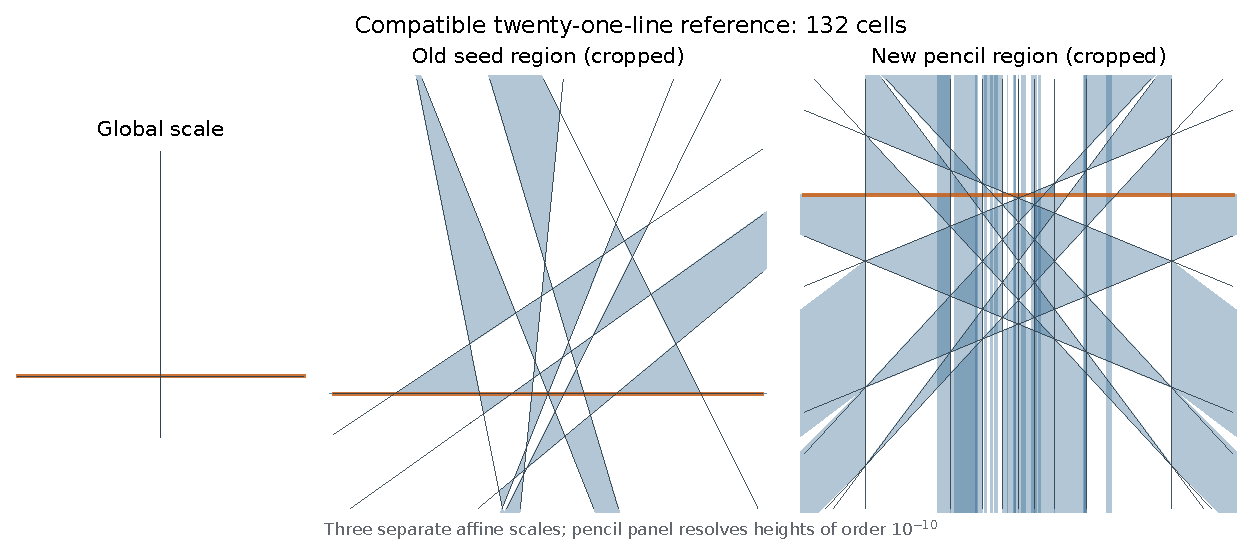
\includegraphics[width=0.88\linewidth]{figures/seed-21.pdf}
\caption{A 21-line hybrid checkpoint with 132 triangles.  The finite
global, core, and thin-pencil views illustrate the scale separation.
The finite rendering is distinct from the true-tangent-grid parametric theorem in
\texttt{BBLSeed21}, which establishes 132 triangles and all 19
distinguished triangles throughout its positive parameter interval.}
\label{fig:seed21}
\end{figure}

Nevertheless, a lower-bound existential statement forgets data needed
by the next step.  The theorem in the library cannot be iterated merely
by substituting its numerical conclusion back into its hypotheses.
The remaining integration has a precise, limited form:
\begin{enumerate}
\item Retain the constructed slopes, the duplicate-free triangle list,
simplicity, distinguished-line saturation, and positive central height
in a recursive seed object.  Select $\kappa$ to preserve the central
triangle independently of the counted list, since that list may omit it.
\item Sort the old and new intercepts into the next grid.  The explicit
permutation and tangent-cut identity are proved in
\texttt{BBLGridReindex}.  The next distinguished triangles are proved
in \texttt{BBLNextSaturation}: each noncentral interval is one of the
mixed triangles, and the central interval uses the retained central
triangle.  Whole-list transport must still supply all support
permutations, preserve distinctness and length, and identify the
reindexed graph equations.
\item Normalize the grouped labels of \texttt{BBLSeed21} into increasing
intercept order.  Its central source labels are 5 and 6, whose apex has
height $5\varepsilon/2$, so positivity follows without another interval
search.  The sorting permutation leaves the central old supports in
place geometrically; hence the next central apex is exactly the old
one, not merely close to it.
\item Induct on a uniform small-parameter existence statement
\begin{equation}
 \exists\eta>0\quad\forall\varepsilon\in(0,\eta)\quad
 \exists\text{ a compatible counted seed at }(q,\varepsilon).
 \label{fam:recursive-quantifier}
\end{equation}
At the next stage shrink $\eta$ below the needed half-grid gap.  The
slopes, $\delta$, and $\kappa$ may depend on $\varepsilon$.
\end{enumerate}
The sought closure is, schematically,
\[
 \operatorname{Compatible}(r,\varepsilon,T)
 \Longrightarrow
 \operatorname{Compatible}(2r,\varepsilon,T+(4r)^2)
\]
under $r\geq5$ and \eqref{fam:epsilon}.  This is a proposed theorem
interface, not a declaration already present in the checked library.
Starting from 21 lines would give the formal target
\begin{equation}
 q_t=20\cdot2^t,\qquad
 \Ks(q_t+1)\geq\frac{q_t^2-4}{3}.
 \label{fam:21-target}
\end{equation}
Numerically this is the tail of \eqref{fam:eleven-family}.  Its purpose
is to close the formal geometric dependency, not to establish another
numerical priority claim.  The stronger even family further requires
the separate visibility invariant of
Proposition~\ref{fam:even-conditional}.

A bounded search for a compatible perfect 21-line seed did not improve
132: it tested 11547910 floating proposals, with exact checking reserved
for any prospective 133-triangle result, and found none.  A separate
3234-program linear-feasibility transfer search likewise found no strict
feasible margin.  These are reproducible negative search results,
consistent with the compatibility difficulties discussed in
\cite{parpalakutkin2026}; neither proves nonexistence.  Improving a
compatible seed, finding a useful partial-doubling interpolation, and
closing the recursive invariant remain different research problems.
